\subsection{LDraw}\label{reserse-ldraw}  
   
LDraw je otevřený standard pro LEGO \gls{CAD} programy, které uživateli umožňují vytvářet virtuální modely a scény. Je možné ho použít k~dokumentaci stavebnic, které jste fyzicky postavili, k~vytvoření stavebních pokynů jako od společnosti LEGO, k~vykreslení 3D fotorealistických obrázků virtuálních modelů a dokonce i k~vytvoření animace. \autocite{ldraw:homepage}  

Podle \autocite[s.~30]{legobook} se systém LDraw skládá ze tří základních částí, které se navzájem doplňují. Těmito částmi jsou: 

\begin{itemize}
    \item souborový formát LDraw,
    \item knihovna součástek,
    \item programy pro tvorbu modelů. 
\end{itemize}

Pro tvorbu mé bakalářské práce jsou důležité pouze první dvě zmíněné součásti systému LDraw. Obě části nyní podrobně analyzuji a zjištěné skutečnosti později uplatním při návrhu doménového modelu aplikace a mechanizmu načítání dat do mé aplikace v~kapitole \emph{\ref{kapitola-navrh}}.
    
\begin{figure}[htbp]
        \centering
        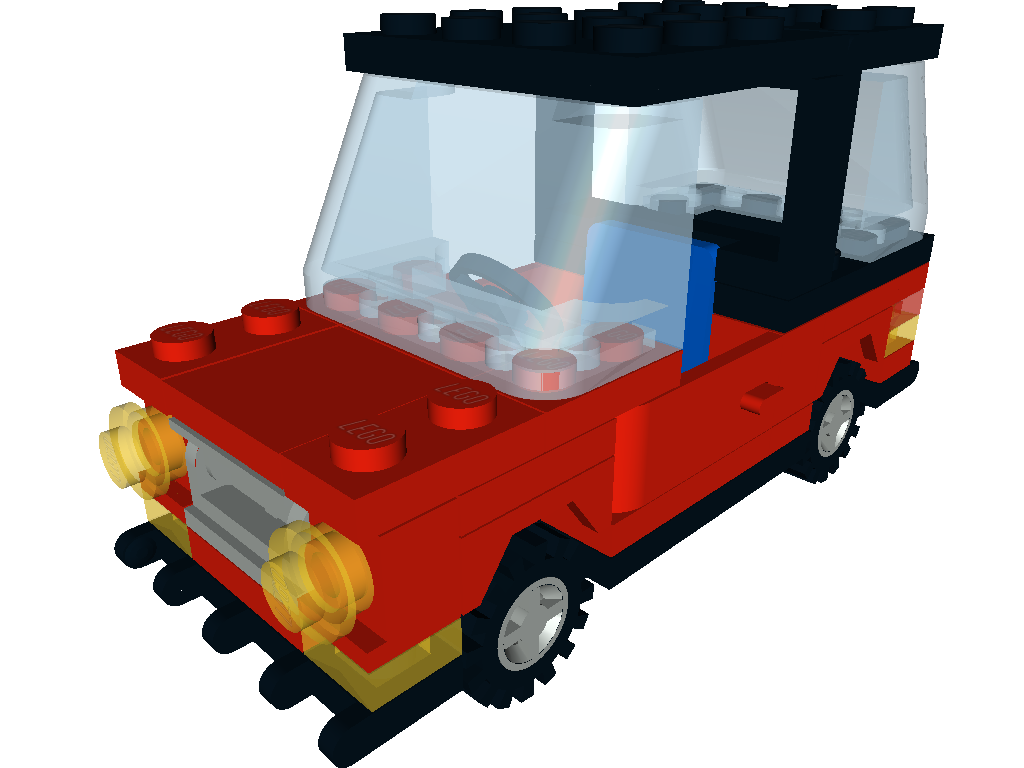
\includegraphics[width=0.6\textwidth,height=\textheight,keepaspectratio]{images/car.png}
        \caption{Ukázkový model z knihovny LDraw \autocite{ldraw:car}}
\end{figure}

    \subsubsection*{Formát LDraw}\label{ldraw-format}
    
    Základním stavebním kamenem, kolem kterého je postavený celý systém LDraw, je stejnojmenný souborový formát LDraw. Soubory v~tomto formátu slouží jak k~ukládání jednotlivých součástek, tak i k~ukládání celých stavebnic. Soubory jednotlivých tvarů, ze kterých se součástky skládají a zároveň součástky samotné mají typicky příponu \textit{DAT}, pro celé stavebnice (skládající se z~více součástek) se používá přípona \textit{LDR}.
    
    Všechny soubory LDraw se řídí pravidly podle oficiální dokumentace, která je dostupná na \autocite{ldraw:file:documentation}. Tato pravidla v~následujících odstavcích ve zjednodušené podobě představím.

        \paragraph{Parsování}\mbox{}

        Soubory ve formátu LDraw jsou dle specifikace \autocite{ldraw:file:specification} textové v~kódování \gls{UTF-8}. Skládají se z~předem neurčeného množství příkazů, přičemž každý řádek odpovídá právě jednomu příkazu.

        Typ příkazu na řádce je určen prvním znakem, který se na ní vyskytuje (s~výjimkou bílých znaků\footnote{Bílý znak je dle specifikace \autocite{ldraw:file:specification} definován jako jedna nebo více mezer, znaků tabulátoru nebo jejich kombinace.}). Možné typy řádků jsou následující: 
        
        \begin{enumerate}
            \item[0:] \textbf{komentář nebo META příkaz}

            \item[1:] \textbf{reference na jiný soubor}

                Příkaz: \mintinline{text}{1 <colour> x y z a b c d e f g h i <file>}, kde: 
                \begin{itemize}
                    \item \mintinline{text}{<colour>} je id barvy specifikované v~\autocite{ldraw:colors},
                    \item \mintinline{text}{x y z} jsou souřadnice pro umístění součástky,
                    \item \mintinline{text}{a b c d e f g h i} je levá horní $ 3\times3 $ matice standardní $ 4\times4 $ homogenní transformační matice,
                    \item \mintinline{text}{<file>} je jméno vkládaného souboru.
                \end{itemize}
                
            \item[2:] \textbf{úsečka}
            \item[3:] \textbf{trojúhelník}
            \item[4:] \textbf{čtyřúhelník}
            \item[5:] \textbf{volitelná úsečka}
        \end{enumerate}

        V~ukázce kódu \emph{\ref{ukazka-soucastky-ldraw}} můžeme vidět příklad jednoduché součástky ve formátu LDraw. Tuto vyrenderovanou součástku je možné vidět na obrázku \emph{\ref{obrazek-ldraw-soucastka}}.
            
       \begin{listing}[htbp]
            \begin{minted}{text}
0 Brick  2 x  2
0 Name: 3003.dat
0 Author: James Jessiman
0 !LDRAW_ORG Part UPDATE 2002-03
0 !LICENSE Redistributable under CCAL version 2.0 : see CAreadme.txt

0 BFC CERTIFY CCW

0 !HISTORY 2001-10-26 [PTadmin] Official Update 2001-01
0 !HISTORY 2002-05-07 [unknown] BFC Certification
0 !HISTORY 2002-06-11 [PTadmin] Official Update 2002-03
0 !HISTORY 2007-05-07 [PTadmin] Header formatted for Contributor
0 !HISTORY 2008-07-01 [PTadmin] Official Update 2008-01

1 16 0 4 0 1 0 0 0 -5 0 0 0 1 stud4.dat

0 BFC INVERTNEXT
1 16 0 24 0 16 0 0 0 -20 0 0 0 16 box5.dat

4 16 20 24 20 16 24 16 -16 24 16 -20 24 20
4 16 -20 24 20 -16 24 16 -16 24 -16 -20 24 -20
4 16 -20 24 -20 -16 24 -16 16 24 -16 20 24 -20
4 16 20 24 -20 16 24 -16 16 24 16 20 24 20

1 16 0 24 0 20 0 0 0 -24 0 0 0 20 box5.dat

1 16 10 0 10 1 0 0 0 1 0 0 0 1 stud.dat
1 16 -10 0 10 1 0 0 0 1 0 0 0 1 stud.dat
1 16 10 0 -10 1 0 0 0 1 0 0 0 1 stud.dat
1 16 -10 0 -10 1 0 0 0 1 0 0 0 1 stud.dat
0
            \end{minted}
            \caption{Ukázka součástky ve formátu LDraw \autocite{ldraw:model}\label{ukazka-soucastky-ldraw}}
        \end{listing}
  
        \begin{figure}[htbp]
            \centering
            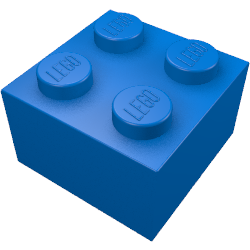
\includegraphics[width=0.3\textwidth,height=\textheight,keepaspectratio]{images/3003.png}
            \caption{Vyrenderovaná součástka z~ukázky kódu \emph{\ref{ukazka-soucastky-ldraw}} \autocite{rebrickable:part:image:3003}\label{obrazek-ldraw-soucastka}}
        \end{figure}

    \subsubsection*{Knihovna LDraw}\label{ldraw-knihovna}
    Knihovna LDraw poskytuje velké množství\footnote{V době psaní práce obsahuje knihovna 9 781 součástek.} 3D modelů LEGO součástek ve formátu LDraw.

    Součástky z~knihovny je možné obdržet jednotlivě z~adresy \url{http://www.ldraw.org/library/official/filepath}, kde \url{filepath} je cesta k~souboru v~knihovně LDraw \autocite{ldraw:download}. Další možností je obdržení kompletní knihovny v~podobě ZIP archivu. Struktura obsahu tohoto archivu je zobrazena na diagramu adresářové struktury \emph{\ref{ldraw-archiv}}.

    \begin{dirfigure}%
        \dirtree{%
            .1 models\DTcomment{složka, do které jsou ukládány vytvořené modely}.
            .1 p \DTcomment{primitiva používaná při tvorbě modelů}.
            .1 parts\DTcomment{kompletní součástky}.
                .2 *.dat\DTcomment{soubory součástek}.
                .2 s\DTcomment{často používané společné části součástek}.
            .1 CAlicense.txt\DTcomment{licenční podmínky}.
            .1 CAreadme.txt\DTcomment{vysvětlení licenčních podmínek}.
            .1 LDConfig.ldr\DTcomment{definice barev}.
            .1 Readme.txt\DTcomment{popis obsahu archivu}.
            .1 mklist.exe\DTcomment{program MKList k~vytvoření seznamu součástek}.
            .1 mklist1\_6.zip\DTcomment{archiv se zdrojovým kódem programu MKList}.
        }
        \caption{Obsah archivu complete.zip}\label{ldraw-archiv}
    \end{dirfigure}

    Aby byla vytvořená součástka přidána do oficiální knihovny LDraw, musí projít schvalovacím procesem. V~tom je kontrolováno dodržení všech pravidel specifikace formátu \autocite{ldraw:file:specification} i další pravidla platná pro knihovnu \cite{ldraw:library:restrictions}.

    \subsubsection*{Hlavička souboru}\label{ldraw-hlavicka}
        Každý LDraw soubor, který se nachází v~knihovně, musí obsahovat hlavičku s~obsahem řídícím se pravidly \autocite{ldraw:header:specification}. V~hlavičce souboru jsou uložena metadata poskytující doplňující informace o~součástce. Mezi tyto informace mimo jiné patří:
        \begin{itemize}
            \item název,
            \item autor,
            \item licence,
            \item typ součástky,
            \item klíčová slova,
            \item kategorie.
        \end{itemize}
 
    \subsubsection*{Typy prvků}\label{ldraw-typy-soucastek}
    V~knihovně se nachází prvky několika různých typů. Specifikace je v~tomto ohledu velmi rozsáhlá \autocite{ldraw:header:specification}\autocite{ldraw:sticker:specification}. Typ prvku je možné rozpoznat podle: 
    \begin{itemize}
        \item názvu (první řádek souboru LDraw),
        \item META příkazů hlavičky,
        \item čísla (jméno souboru).
    \end{itemize}
    
    Po detailním prozkoumání většího množství prvků musím podotknout, že ne všechny soubory knihovny přesně odpovídají specifikaci. 

    Možné typy prvků:
    
    \begin{itemize}
        \item \textbf{Part:} Geometricky kompletní součástka.
        \item \textbf{Subpart:} Sám o~sobě nekompletní útvar.
        \item \textbf{Primitive:} Základní geometrický útvar vyskytující se v~mnoha součástkách.

        Pro více informací o~primitivech a jejich kompletní seznam doporučuji \autocite{ldraw:primitives}.

        \item \textbf{Shortcut:} Součástka složená z~více kompletních součástek.

        Na obrázku \emph{\ref{obrazek-ldraw-shortcut}} je možné vidět render součástky \textit{3015c01} (nahoře) skládající se ze součástek \textit{3815}, \textit{3816}, \textit{3817} (dole).

        \item \textbf{Alias:} Soubor odkazující na jiné místo v~knihovně (například z~důvodu používání dvou různých čísel pro stejný prvek společností LEGO). 
        
        Soubor typu \textit{Alias} typicky obsahuje pouze jeden příkaz typu \text{1}. Náhled souboru typu \textit{Alias} je k~vidění v~ukázce kódu \emph{\ref{ukazka-alias}}.

        \item \textbf{Physical\_Colour:} Soubor odkazující na jiné místo v~knihovně a navíc určující barvu.
        \item \textbf{Sticker:} Potisk.
        \item \textbf{Patterned:} Součástka s~potiskem.
        
        Porovnání součástky typu \textit{Part} a odpovídající součástky typu \textit{Patterned} je vidět na obrázku \emph{\ref{obrazek-ldraw-patterned}}.
        
    \end{itemize}
   
    \begin{figure}[htbp]
        \centering
        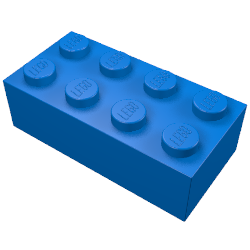
\includegraphics[width=0.3\textwidth,height=\textheight,keepaspectratio]{images/3001.png}
        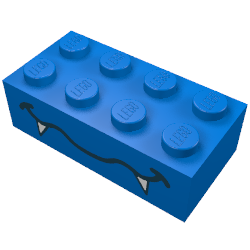
\includegraphics[width=0.3\textwidth,height=\textheight,keepaspectratio]{images/3001p0b.png}
        \caption{Ukázka součástky typu \textit{Part} a \textit{Patterned} \autocite{rebrickable:part:image:3001}\autocite{rebrickable:part:image:3001p0b}\label{obrazek-ldraw-patterned}}
    \end{figure}

      \begin{listing}[htbp]
        \begin{minted}{text}
0 ~Moved to 6141
0 Name: 4073.dat
0 Author: [PTadmin]
0 !LDRAW_ORG Part Alias UPDATE 2015-01
0 !LICENSE Redistributable under CCAL version 2.0 : see CAreadme.txt

0 BFC CERTIFY CCW

0 !HISTORY 2015-10-11 [PTadmin] Official Update 2015-01

0 // Plate  1 x  1 Round

1 16 0 0 0 1 0 0 0 1 0 0 0 1 6141.dat
        \end{minted}
        \caption{Ukázka souboru typu \textit{Alias} \autocite{ldraw:model:alias}\label{ukazka-alias}}
    \end{listing}

    \begin{figure}[htbp]
        \centering
        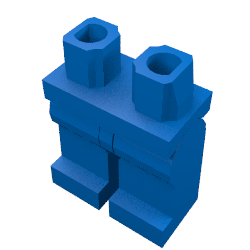
\includegraphics[width=0.4\textwidth,height=\textheight,keepaspectratio]{images/3815c01.png}
        \\
        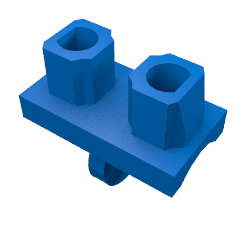
\includegraphics[width=0.3\textwidth,height=\textheight,keepaspectratio]{images/3815.png}
        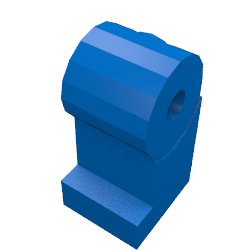
\includegraphics[width=0.3\textwidth,height=\textheight,keepaspectratio]{images/3816.png}
        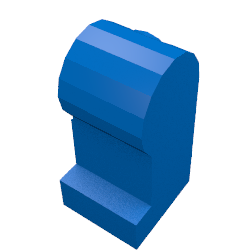
\includegraphics[width=0.3\textwidth,height=\textheight,keepaspectratio]{images/3817.png}
        \caption{Ukázka součástky typu \textit{Shortcut} \autocite{rebrickable:part:image:970c00}\autocite{rebrickable:part:image:3815}\autocite{rebrickable:part:image:3816}\autocite{rebrickable:part:image:3817}\label{obrazek-ldraw-shortcut}}
    \end{figure}

    % Pravidla pojmenovávání jednotlivých souborů s~ohledem na jejich typ jsou znázorněna v~tabulce \emph{\ref{tabulka-ldraw-cislovani}}.

    % \begin{table}[th!]
    % \centering
    %     \caption{Shrnutí pravidel pro číslování součástek \autocite{ldraw:numbering:faq}}
    %     \label{tabulka-ldraw-cislovani}
    %     \begin{tabularx}{\textwidth}{@{}rX@{}}
    %     \toprule
    %     Vzor pojmenovávání & Typ prvku
    %     \\ \midrule
    %     nnn, nnnn, nnnnn & \textit{Part}
    %     \\
    %     <number>Cnn & \textit{Shortcut}
    %     \\
    %     <number>Dnn & kombinace \textit{Part} a \textit{Sticker}
    %     \\
    %     <number>Pxx & \textit{Patterned} 
    %     \\
    %     s/<number> & \textit{Subpart} (umístěná ve složce parts/s)
    %     \\
    %     <number>a & Novější verze součásky <number>
    %      \\
    %     \bottomrule
    %     \multicolumn{2}{l}{n = číslice, x = číslice/písmeno, a = písmeno}
    %     \\
    %     \multicolumn{2}{l}{<number> = kompletní pojmenovávání jiného prvku}
    %     \end{tabularx}
    % \end{table}

    \subsubsection*{Licence}\label{ldraw-licence}
    Všechny součástky zahrnuté do oficiální knihovny LDraw jsou vydány pod licencí \gls{CC-BY} \autocite{CC-BY}. Ta umožňuje úpravu i sdílení díla za předpokladu dodržení podmínky o~uvedení autora, licence a označení případných provedených změn.

    % \subsubsection{Závěr}\label{ldraw-zaver}
    %TODO
    
    %  Součástky navíc obsahují doplňující informace, pomocí kterých je možné je třídit a vyhledávat. 